\documentclass[10pt,twocolumn,letterpaper]{article}
\usepackage{graphicx}
\graphicspath{ {./} }

\begin{document}

%%%%%%%%% TITLE
\title{Predicting a Film's Rating Utilizing Machine Learning}

\author{Joel Martinez\\
Texas State University\\
\and
Jose Garcia\\
Texas State University\\
\and
Kameron Bush\\
Texas State University\\\\
}
\maketitle
%\thispagestyle{empty}

%%%%%%%%% ABSTRACT
\begin{abstract}
	We present a program that will utilize existing data on films that have been released in order to predict
	the rating of a film that has yet to be released. This prediction will be given to the film industries that created the film in order to give them a chance to improve the film if needed. The factors being used are IMDB rating, budget, USA gross, USA opening weekend gross, tomatometer, metascore, and worldwide gross. We used using linear regression as the model for the project and it will be optimized using the k-fold method.
\end{abstract}

%%%%%%%%% BODY TEXT
\section{Problem Description}
	When a film industry decides to create a film, the creators have to factor in many attributes that are important to how the public will interpret and perceive the film. Some of these factors are the company’s film budget, the film critic ratings, and how much the film makes on its first weekend.\\
	This public interpretation is very important to the film company because how the public perceives the film ultimately determines how many people go and see the film. The amount of people who go see the movie ultimately determines if the film company makes a profit off of the movie, i.e. if it is a ‘hit’ or a ‘flop’.\\
	The fate of the film cannot be determined until after the film is released to the public making it too late to make any changes if it fails. Our program is aimed to fix this problem by analyzing factors of previous films in order to predict the audience rating the new film will receive. This audience rating will give the film company a general idea of how well their film will do before they release the movie. Based on the audience rating presented, the film company will be able to fix their film before release so they can maybe save the film from flopping.

%-------------------------------------------------------------------------
\section{Survey}
	To see how much of an impact this project would have with the general population, we asked 50 students their opinion.\\\\
	Q: Do you believe this project will have an impact on which movies you will watch based on the rating generated?\\\\
	37 students said it would have an impact.\\
	9 students said it would not impact them.\\
	4 students said they did not know.

%-------------------------------------------------------------------------
\section{Plan}
	March 8th - Understand the Problem in-depth\\
	- Our group has got a now gotten a better understanding of how we can attack this problem. Our attributes will be able to help us use our model to estimate the probability of success (IMBD Rating, Budget, USA Gross, USA Opening Weekend Gross, Tomatometer, Metascore, Worldwide Gross).\\\\
	March 14th - Develop a data base for the code\\
	- We first created a database where we stored our x attributes and our y audience rating (1.0-10.0) in excel.\\\\
	March 25th - Complete a base algorithm for Project\\
	- Our model first takes the data from the database (excel), then splits our data to a X and Y dataset. Our model will consist of a train/test split of the X and Y dataset. We used Linear Regression to find a relation between the X attributes and the rating, we then proceeded to use the K-Fold method to optimize our model.\\\\
	March 29th - Complete Intermediate Project Report\\
	- Done and done.\\\\
	April 10th - Research ways to make algorithm more accurate\\
	- Yet to be done.\\\\
	April 20th - Edit algorithm to be more effective and more precise\\
	- Yet to be done.\\\\
	April 29th - Complete Final Project Presentation\\
	- Yet to be done.\\\\
	May 4th - Complete Final Project Report\\
	- Yet to be done.

%-------------------------------------------------------------------------
\section{Data}
	The data set contains seven attributes (or features, denoted by X1. . . X8) and
	one response (or outcomes, denoted by y1). The aim is to use these seven
	features to predict the outcome.\\
	We specifically choose these seven features because the information is easy to find
	and open to the public. Some other attributes that we considered for the data was
	harder to come across on the internet and left many holes in our data. This would have
	required us to have to clean our data beforehand. With the attributes we are using
	there is no need to clean the data because we handpicked each movie individually to
	contain all or most of the attributes.\\
	Data was obtained from the Rotten Tomatoes website which provided us with the
	Tomatometer (Rotten Tomatoe's score of the movie), and the audience score (the value
	that we intend to predict.) We also utilized the IMDb website to obtain the gross USA
	(the amount of money that was made in the USA), the gross opening weekend USA (the amount
	of money that was made in the first week that the movie was released to the public),
	worldwide gross (the total amount of money made around the globe), budget (the amount of
	money the studio spent to create the movie), metascore (the IMDb user's score of the
	film), and IMDb rating (the score that IMDb critics gave the film.)
	\\\\Specifically:\\
	\\*X1 Gross USA\\
	\\*X2 Gross Opening Weekend USA\\
	\\*X3 Worldwide Gross\\
	\\*X4 Budget\\
	\\*X5 Metascore\\
	\\*X6 IMDb rating\\
	\\*X7 Tomatometer\\
	\\*y1 Audience Score\\\\
	
	Below is a screenshot of the first few lines in the dataset that we are utilizing for our
	model. As you can see, most attributes are filled in and few are null. We intend to expand
	the size of of the dataset as we continue to work on the project. Much of the data is gathered
	by hand and requires a large amount of time to find.\\
	
	\begin{center}
	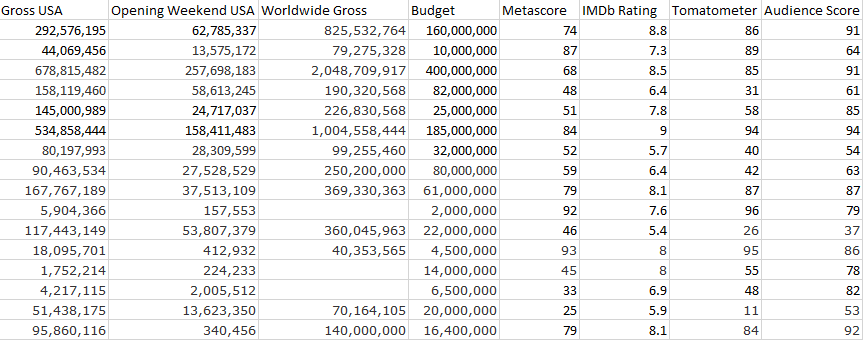
\includegraphics[scale=0.78]{moviedatashot}
	\end{center}

%-------------------------------------------------------------------------

%%%%%%%%% BIBLIOGRAPHY
\begin{thebibliography}{9}
	\bibitem{latexcompanion} 
	Quader, Nahid \& Gani, Md. \& Chaki, Dipankar \& Ali, Md. 
	\textit{A Machine Learning Approach to Predict Movie Box-Office Success}. 
	Reading, Bangladesh, 2018.
	
	\bibitem{latexcompanion} 
	Sharda, Ramesh \& Delen, Dursun 
	\textit{Predicting box-office success of motion pictures with neural networks}. 
	Expert Systems with Applications. 30. 243-254. 10.1016/j.eswa.2005.07.018.
	
	\bibitem{latexcompanion} 
	B. R. Litman \& H. Ahn
	\textit{Predicting financial success of motion pictures}.
	In B. R. Litman (Ed.), the motion picture mega-industry. Boston, MA: Allyn \& 
	Bacon Publishing, Inc. (1998)
	
	\bibitem{latexcompanion}
	M.H Latif \& H. Afzal
	\textit{Prediction of Movies popularity Using Machine Learning Techniques}.
	National University of Sciences and technology, H-12, ISB, Pakistan. 
\end{thebibliography}

\end{document}
